\documentclass[12pt]{amsart}
\setlength{\marginparwidth}{0.5in}
\usepackage{amsmath,amssymb,natbib,graphicx}
\textheight 9in
\textwidth 6.5 in
\hoffset -1 in
\voffset -1 in
\input FJHDef.tex

\newcommand{\sphere}{\mathbb{S}}
\newcommand{\cc}{\mathcal{C}}
\newcommand{\cq}{\mathcal{Q}}
\newcommand{\bbW}{\mathbb{W}}
\newcommand{\tP}{\widetilde{P}}
\newcommand{\bg}{{\bf g}}
\newcommand{\bu}{{\bf u}}
\newcommand{\bbu}{\bar{\bf u}}
\newcommand{\bv}{{\bf v}}
\newcommand{\bbv}{\bar{\bf v}}
\newcommand{\bw}{{\bf w}}
\newcommand{\bbw}{\bar{\bf w}}
\newcommand{\hv}{\hat{v}}
\newcommand{\fudge}{\mathfrak{C}}
\DeclareMathOperator{\MSE}{MSE}
\DeclareMathOperator{\RMSE}{RMSE}
\DeclareMathOperator{\rnd}{rnd}
\DeclareMathOperator{\abso}{abs}
\DeclareMathOperator{\rel}{rel}
\DeclareMathOperator{\nor}{nor}
\DeclareMathOperator{\err}{err}
\DeclareMathOperator{\prob}{prob}
\DeclareMathOperator{\third}{third}
%\DeclareMathOperator{\fourth}{fourth}
\newtheorem{theorem}{Theorem}
\newtheorem{prop}[theorem]{Proposition}
\DeclareMathOperator{\sMC}{sMC}
\DeclareMathOperator{\aMC}{aMC}
\begin{document}

\title{Adaptive Simple Monte Carlo}
\author{Fred J. Hickernell}
\author{Lan Jiang}
\author{Yuewei Liu}
\address{Room E1-208, Department of Applied Mathematics, Illinois Institute of Technology, 10 W.\ 32$^{\text{nd}}$ St., Chicago, IL 60616}
\address{Room E1-208, Department of Applied Mathematics, Illinois Institute of Technology, 10 W.\ 32$^{\text{nd}}$ St., Chicago, IL 60616}
\address{School of Mathematics and Statistics, Lanzhou University, Lanzhou City, Gansu, China 730000}
\begin{abstract}We attempt a probabilistic analysis of simple Monte Carlo, achieving probabilistic error bounds when the kurtosis is controlled.  The algorithm uses a sample size that depends adaptively on the estimated variance of the integrand.  Thus, the algorithm is nonlinear (depending essentially on the function).  The advantage of what is done here over standard error analysis (complexity theory) is that the algorithm does not depend a priori on the scale of the problem (in this case the variance) to determine the number of samples.   Our intention, if what is done here is correct, is to try to extend this to the more sophisticated sampling schemes and infinite dimensional problems.
\end{abstract}
\maketitle


\section{Introduction}

When one tries to utilize theoretical error bounds or complexity results for Monte Carlo integration to inform a practical algorithm, there are some real challenges.  To determine the sample size needed, one must have some information about the size of the function, specifically its standard deviation in the case of simple Monte Carlo.  Estimating this standard deviation is a step whose error is typically not analyzed.  Moreover, if one wants to guarantee that the answer obtained by the Monte Carlo algorithm satisfies a given error tolerance with a high probability, then in practice one often resorts to Central Limit Theorem, whose application also introduces an additional error that is not well understood.  

This article attempts to address these shortcomings by derving a tight theory that accounts rigorously for as much of the error in a practical algorithm as is possible.  This is done by means of some probability inequalities that involve higher moments and a variant to traditional information-based complexity theory that measures the cost of the problem in terms of the unknown size of the integrand.  

\section{Simple Monte Carlo in Practice}

Suppose one wishes to compute the following integral or mean, $\mu$, of some $d$-variate function $f: \reals^d \to \reals$, i.e.,
\begin{equation*}
\mu= \mu(f) = \int_{\reals^d} f(\vx) \rho(\vx) \, \dif \vx,
\end{equation*}
where $\rho: \reals^d \to [0,\infty)$ is a specified probability density function.  A simple Monte Carlo algorithm to estimate this integral is the sample mean of the function evaluated at independent and identically distributed random variables $\vX_1, \vX_2, \ldots$ with the marginal probability density function $\rho$:
\begin{equation*} %\label{simpleMCest}
\hmu_n = \frac 1n \sum_{i=1}^n Y_i, \qquad Y_i = f(\vX_i).
\end{equation*}

A natural question is the following: \emph{How large should $n$ be to ensure with some reasonable certainty, that the error of the approximation is no larger than some error tolerance, $\varepsilon$?}  In practice, a common approach is to invoke the Central Limit Theorem, which says that for a significance level or uncertainty tolerance, $\alpha$, one has
\begin{equation} \label{CLT}
\Prob\left[\abs{\hmu_n-\mu} \le \frac{z_{\alpha/2} \sigma}{\sqrt{n}} \right] \approx 1-\alpha,
\end{equation}
where $z_\alpha$ denotes the $(1-\alpha)100\%$ percentile of the standard Gaussian distribution, and $\sigma^2$ denotes the variance of the function:
\begin{equation} \label{sigmadef}
\sigma^2 := \var(Y_1) = \var(f(\vX_1)) =: \var(f) = \int_{\reals^d} \abs{f(\vx)-\mu}^2 \rho(\vx) \, \dif \vx.
\end{equation}
This variance $\sigma^2$ can be estimated in terms of the sample variance based on an initial  sample of size, $n_0 \in \naturals$:
\begin{equation} \label{samplevar}
\hsigma^2 = \fudge^2 \hv_{n_0}, \qquad \text{where} \quad \hv_{n_0} = \frac 1{n_0-1} \sum_{i=1}^{n_0} [Y_i- \hmu_{n}]^2, \quad Y_i=f(\vX_i).
\end{equation}
The fudge factor $\fudge>1$ accounts for the fact that as an unbiased estimator, the sample variance may be larger or smaller than the true variance.  Defining 
\begin{equation} \label{CLTsample}
N_{G}(\varepsilon,\alpha) :=\left \lceil \left(\frac{z_{\alpha/2}}{\varepsilon}\right)^2 \right \rceil, 
\end{equation}
in light of the Central Limit Theorem, one then estimates the true mean by $\hmu_{n}$, based on an additional $n=N_{G}(\varepsilon/\hsigma,\alpha)$ independent samples:
\begin{equation} \label{simpleMCest}
\hmu_n = \frac 1n \sum_{i=n_0+1}^{n_0+n} Y_i, \qquad Y_i = f(\vX_i).
\end{equation}
This algorithm has a cost of $n_0+N_{G}(\varepsilon/\hsigma,\alpha)$ function evaluations, which depends on the initial sample size, $n_0$, the error tolerance, $\varepsilon$, the degree of uncertainty, $\alpha$, the fudge factor, $\fudge$, and the sample variance, $\hsigma^2$.

The algorithm defined by \eqref{samplevar}, \eqref{CLTsample}, and \eqref{simpleMCest} is practical.  It is economical because it is adaptive, i.e., it estimates the final sample size necessary to approximate the mean.  Unfortunately, this algorithm is based on two assumptions that require justification or modification:
\begin{enumerate}
\renewcommand{\labelenumi}{\roman{enumi})}
\item the variance of $Y=f(\vX)$ is only known approximately, and
\item the Gaussian approximation for the sample mean given by Central Limit Theorem is only approximately true.
\end{enumerate}
This article proposes to tighten these assumptions.  At the same time a complexity theory is developed that allows the cost of computing the answer to be represented in terms of the unknown size of the function, in this case $\sigma$.


\section{Adaptive Monte Carlo}

First the question of bounding the variance is addressed.  The integrands under consideration are assumed to have finite moments of up to a certain order.  Define the $\cl_{p}$ norm of $f$ as follows:
\[
\norm[p]{f} :=\left\{\int_{\reals^d} \abs{f(\vx)}^p \rho(\vx) \, \dif \vx\right\}^{1/p}
\]
Also define the the absolute centered $p^{\text{th}}$ moment of $f$ as
\begin{equation} \label{momentdef}
M_p(f) := \int_{\reals^d} \abs{f(\vx)-\mu}^p \rho(\vx) \, \dif \vx = \norm[p]{f - \mu}^p, \qquad p \ge 1
\end{equation}
By these definitions, the variance of $Y_1$ is the second moment, i.e., $M_2(f) = \var(Y_1)=\sigma^2$, and all functions in $\cl_2$ have finite variance.

As mentioned in \eqref{samplevar}, a practical upper bound on this variance is obtained from the sample variance, $\hsigma^2 = \fudge^2 \hv_{n_0}$, where $\fudge > 1$ is some fudge factor. This can be justified in a probabilistic sense by appealing to  Cantelli's inequality (Theorem \ref{Can}) and the variance of $\hv_{n_)}$ given by Theorem \ref{Varvarthm}.  Proposition \ref{propCant} implies that
\[
\Prob\left[\frac{\hv_{n_0}}{1 - \sqrt{\left ( \kappa  - \frac{n_0-3}{n_0-1}\right)\left(\frac{1-\alpha}{\alpha n_0}\right)}} > \sigma^2 \right] \ge 1 - \alpha,
\]
where $\kappa$ is the \emph{kurtosis} of the integrand:
\begin{equation} \label{kurtdef}
\kappa:= \kurt(f) = \frac{M_4(f)}{\var^2(f)} = \frac{M_4(f)}{\sigma^4} \ge 1 \qquad \forall f \in \cl_4.
\end{equation}
Note that the kurtosis of a function is independent of its scale.  Moreover, functions in $\cl_4$ automatically have finite variance.  It follows that the kurtosis of the integrand must be small enough, relative to $n_0$ and $\fudge$ to ensure that the variance estimate is correct in a probabilistic sense, namely, 
\begin{align}
\nonumber
\frac{1}{1 - \sqrt{\left ( \kappa  - \frac{n_0-3}{n_0-1}\right)\left(\frac{1-\alpha}{\alpha n_0}\right)}}  &\le \fudge^2\\
\nonumber
\frac{1}{\fudge^2} & \le 1 - \sqrt{\left ( \kappa  - \frac{n_0-3}{n_0-1}\right)\left(\frac{1-\alpha}{ \alpha n_0}\right)} \\
\nonumber
\left ( \kappa  - \frac{n_0-3}{n_0-1}\right)\left(\frac{1-\alpha}{ \alpha n_0}\right)   & \le \left(1 - \frac{1}{\fudge^2}\right)^2\\
\kappa  & \le \frac{n_0-3}{n_0-1} + \left(\frac{ \alpha n_0}{1-\alpha}\right) \left(1 - \frac{1}{\fudge^2}\right)^2 =: \kappa_{\max} (\alpha,n_0,\fudge). \label{kappamaxdef}
\end{align}

Figure \ref{kurtmaxfig} shows how large a kurtosis can be accommodated for a given $n$, $\alpha$, and fudge factor $\fudge=1.5$.  Note that for $n=30$, a common rule of thumb for applying the central limit theorem, even $\alpha=0.1$ gives $\kappa_{\max}$ of only about $2$, which is rather restrictive.

\begin{figure}
\centering
\includegraphics[width=3in]{kurtmaxfig.eps}
\caption{The maximum kurtosis, $\kappa_{\max}(n,\alpha,1.5)$, as defined in \eqref{kappamaxdef}. \label{kurtmaxfig}}
\end{figure}

The other issue that needs to be addressed is a tight probabilistic error bound.  The error bound given by the Central Limit Theorem, \eqref{CLT}, is only approximate.   Chebyshev's inequality implies that the number of function evaluations needed to ensure that $\hmu_n$ satisfies the error tolerance with high probability is
\begin{equation} \label{NCdef}
\Prob\left[\abs{\hmu_n-\mu} \le \varepsilon \right] \ge 1-\alpha \quad \text{for } n \ge N_{C}(\varepsilon/\sigma,\alpha), \qquad \text{where }
N_{C}(\varepsilon,\alpha) :=\left \lceil \frac{1}{\alpha\varepsilon^2} \right \rceil.
\end{equation}
However, this sample size is much larger than that given by the Central Limit Theorem, as shown in Figure \ref{alphacomparefig}.

\begin{figure}
\centering
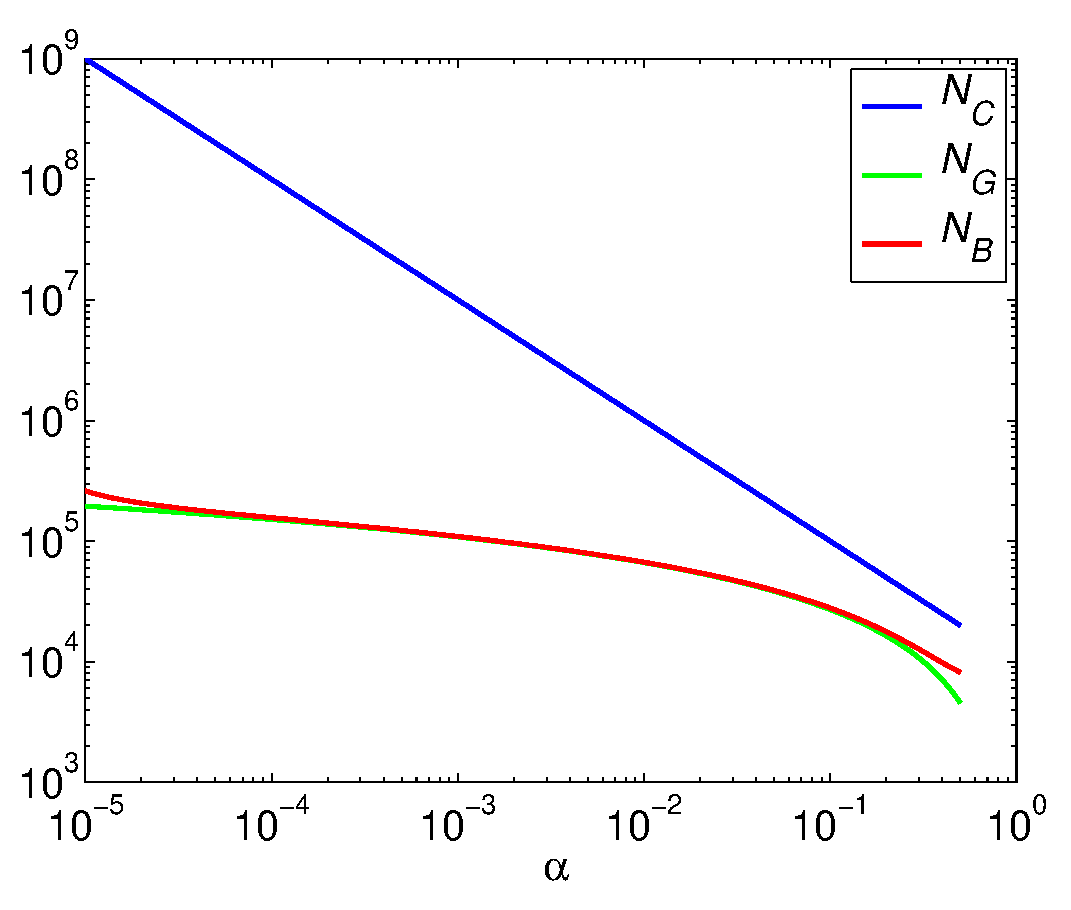
\includegraphics[width=3in]{alphacompare.eps} \quad 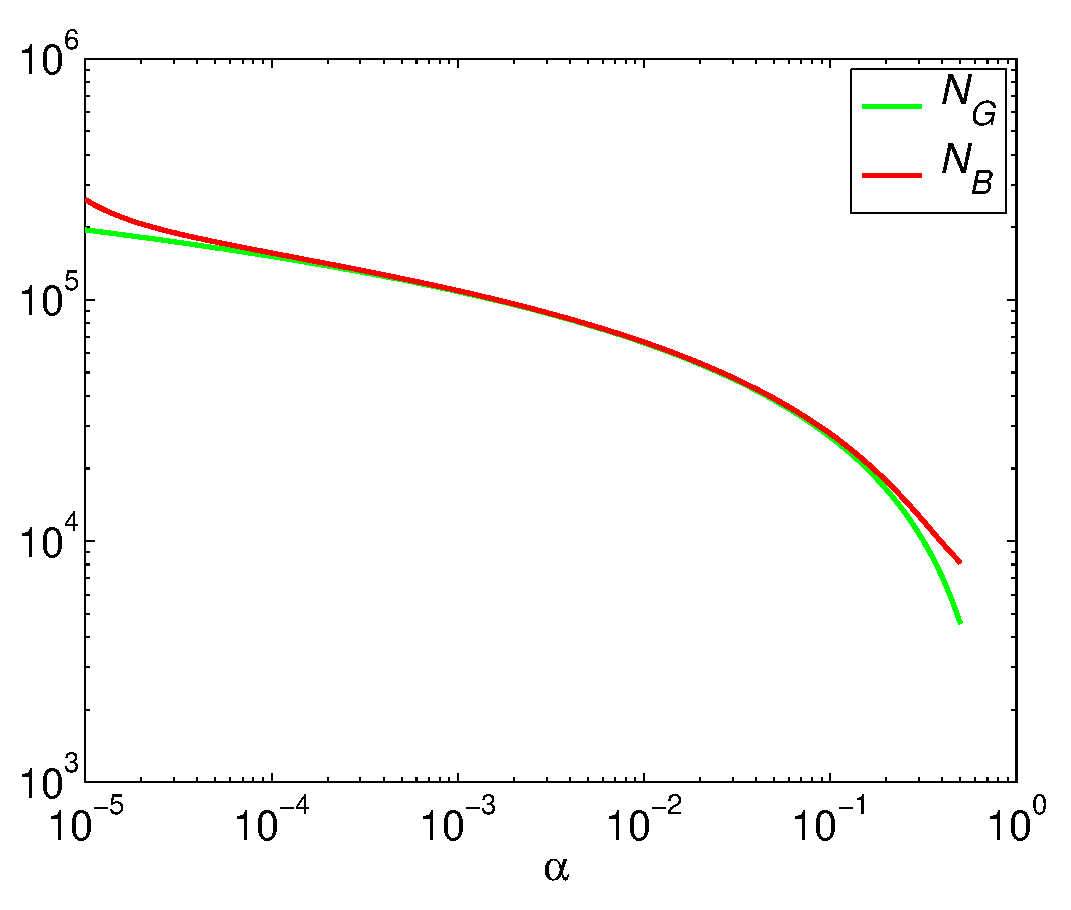
\includegraphics[width=3in]{alphacompareb.eps} \quad 
\caption{Comparison of $ N_G(\varepsilon,\alpha)$, $N_C(\varepsilon,\alpha)$, and $N_B(\varepsilon,\alpha,\varrho)$ for $\varepsilon = 0.001$, and $\varrho=5$. \label{alphacomparefig}}
\end{figure}

Since higher order moments of the integrand are required to guarantee an upper bound on the true variance in terms of the sample variance, it is sensible to use these higher order moments to obtain smaller sample sizes.  A smaller sample size than \eqref{NCdef} with a rigorous probabilistic bound can be
found by invoking the non-uniform Berry-Esseen inequality (Theorem
\ref{BE}). This inequality makes strong assumptions on the
distribution of $f(\vX)$, namely, a finite third moment, $M_3 < \infty$
Recalling that $Y_i = f(\vX_i)$, $\mu=E(Y_i)$, and $\hmu_n =
(Y_1 + \cdots + Y_n)/n$, it then follows by the non-uniform
Berry-Esseen inequality, that
\begin{align*}
\Prob\left[\abs{\hmu_n - \mu} <\frac{\sigma}{\sqrt{n}}x\right]&=\Prob\left[\hmu_n - \mu<\frac{\sigma}{\sqrt{n}}x\right]-\Prob\left[\hmu_n - \mu <-\frac{\sigma}{\sqrt{n}}x\right]\\
&\ge \left[\Phi(x)-A\frac{\varrho}{\sqrt{n}}(1+\abs{x})^{-3}\right] -\left[\Phi(-x) + A\frac{\varrho}{\sqrt{n}}(1+\abs{x})^{-3}\right]\\
&=1-2\left(A\frac{\varrho}{\sqrt{n}}(1+\abs{x})^{-3}+\Phi(-x)\right),
\end{align*}
where $\varrho:=M_3/\sigma^3$, and $\Phi$ is the standard Gaussian cumulative distribution function.  Letting $x=\varepsilon/\varsigma$, the probability of
making an error less than $\varepsilon$ is bounded below by $1-\alpha$, i.e., 
\begin{subequations} \label{proberrcritsampleBE}
\begin{equation}
\Prob[\abs{\hmu_n -\mu}<\varepsilon] \geq 1-\alpha,  \quad \text{provided } n \ge N_B(\varepsilon/\sigma,\alpha,\varrho),
\end{equation}
where 
\begin{equation}\label{NB}
N_B(b,\alpha,\varrho) := \min \left \{ n \in \naturals : \Phi\left(-b \sqrt{n}  \right)+\frac{A\varrho}{\sqrt{n}}\left(1+ b\sqrt{n} \right)^{-3}
\le \frac{\alpha}{2} \right \}.
\end{equation}
\end{subequations}

Definition \eqref{NB} may be re-written implicitly
\begin{equation}\label{NBalt}
N_B = \left \lceil \left(\frac{z_{\alpha/2 -  A
\varrho/(\sqrt{N_B}(1+b\sqrt{N_B})^3)}}{b}\right)^2 \right \rceil.
\end{equation}
The definition of $N_B$ implies that
\[
N_G(b,\alpha) \le N_B(b,\alpha,\varrho) \le \min_{0 \le
\theta \le 1} \left\{\max\left[ \sqrt{\frac{2A
\rho}{\theta\alpha b^3}},
 N_G(b,(1-\theta)\alpha)  \right] \right\}.
\]
Here $A$ is some absolute number \ldots.
As shown in Figure \ref{alphacomparefig}, $N_B$ is close to $ N_G$ for moderate $\alpha$, but $N_B$ may be significantly larger for very small $\alpha$.  In general $N_B$ is smaller than $N_C$.  The disadvantage of \eqref{probcostBE} is that class of integrands is smaller than that in \eqref{probcostCheb}, but this typically a small price to pay given the much smaller cost of computation.

\begin{figure}
\centering
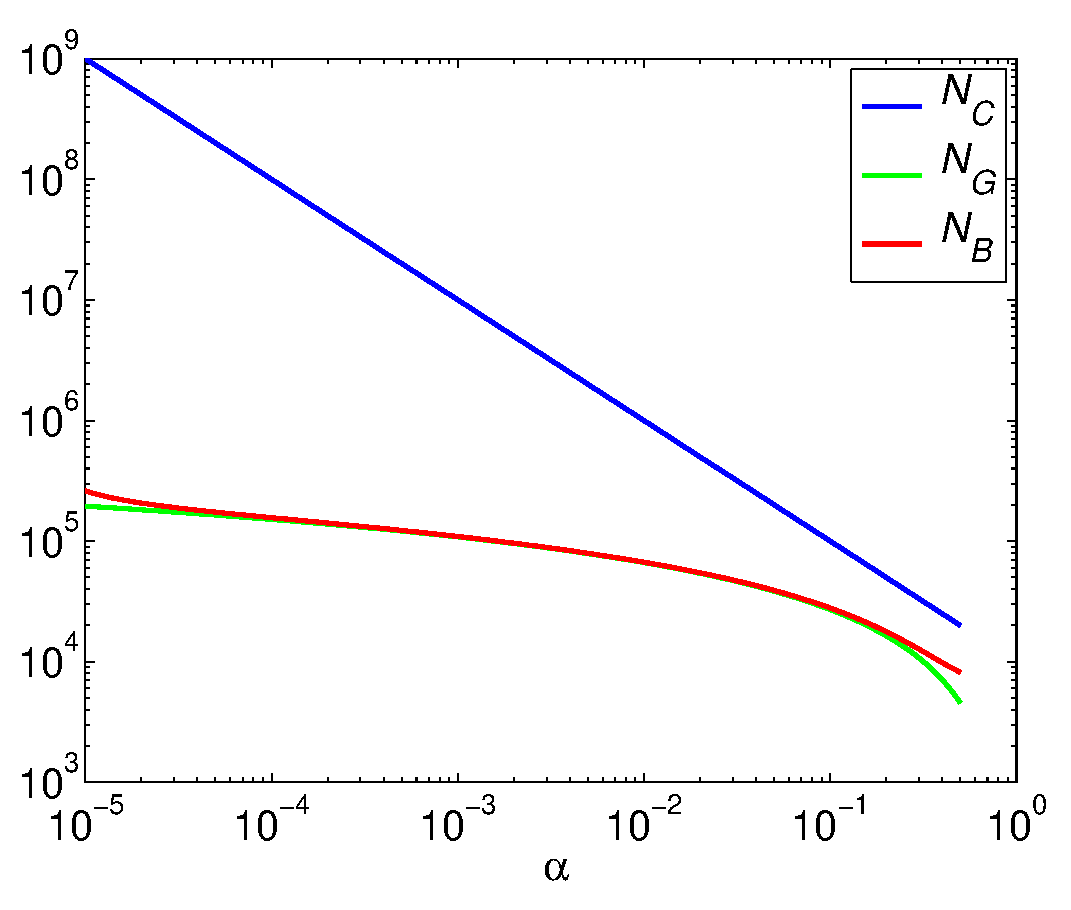
\includegraphics[width=3in]{alphacompare.eps} \quad 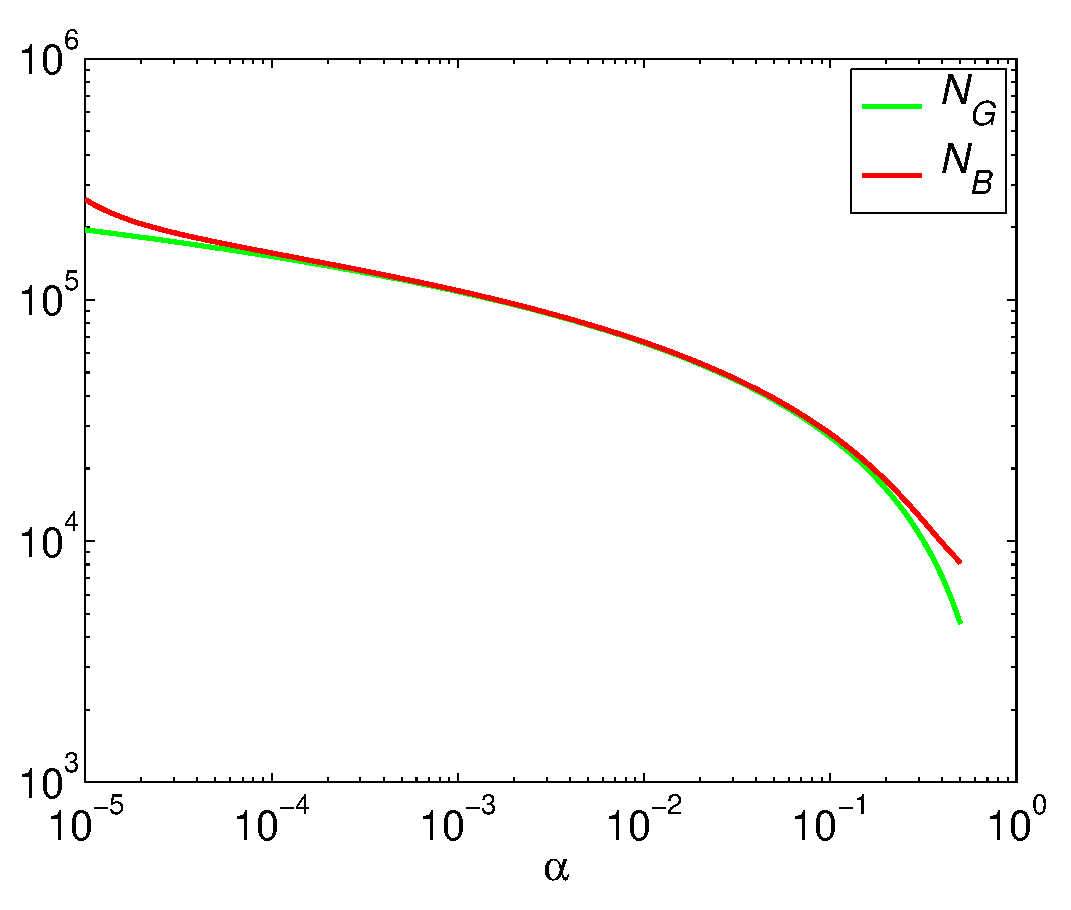
\includegraphics[width=3in]{alphacompareb.eps} \quad 
\caption{Comparison of $ N_G(\varepsilon,\alpha)$, $N_C(\varepsilon,\alpha)$, and $N_B(\varepsilon,\alpha,\varrho)$ for $\varepsilon = 0.001$, and $\varrho=5$. \label{alphacomparefig}}
\end{figure}

The error analyses of the simple, non-adaptive Monte Carlo method has some practical shortcomings.  To apply the randomized or probabilistic cases one must have some a priori knowledge of $\sigma^2$, the variance of the integrand.  It must not larger than $\sigma^2_{\max}$ or the theory does not apply.  If the variance of the integrand is much smaller than $\sigma^2_{\max}$, then the specified sample sizes, 
\[
\left\lceil \frac{\sigma^2_{\max}} {\varepsilon^2} \right \rceil \text{ in  \eqref{randcostsMC}}, \qquad N_{C}(\varepsilon/\sigma_{\max},\alpha) \text{ in  \eqref{probcostCheb}, or} \qquad  N_{B}(\varepsilon/\sigma_{\max},\alpha,\varrho_{\max}) \text{ in  \eqref{probcostBE}}, \qquad
\]
are much too large.  To overcome this shortcoming requires an adaptive Monte Carlo algorithm that estimates the sample size based on the sample variance, as suggested in the introduction.

\section{Adaptive Monte Carlo}

In practice one typically uses observed function values observed to approximate $\sigma^2$ by the sample variance, as follows:
\begin{equation} \label{samplevar}
\hv_{n} = \frac 1{n-1} \sum_{i=1}^{n} [f(\vX_i)- \hmu_{n}]^2.
\end{equation}
To ensure that one does not underestimate the variance, and thus the needed sample size, one might choose to approximate the variance by $\hsigma^2_n = L^2 \hv_n$, where $L > 1$ is some fudge factor. This can be formalized in a probabilistic sense by appealing to  Cantelli's inequality (Theorem \ref{Can}) and the variance of $\hv_n$ in Theorem \ref{Varvarthm}.  Proposition \ref{propCant} implies that
\[
\Prob\left[\frac{\hv_n}{1 - \sqrt{\left ( \kappa  - \frac{n-3}{n-1}\right)\left(\frac{1-\alpha}{\alpha n}\right)}} > \sigma^2 \right] \ge 1 - \alpha,
\]
where
\begin{equation} \label{kurtdef}
\kappa:= \kurt(f) = \frac{M_4(f)}{\var^2(f)} = \frac{M_4(f)}{\sigma^4} \ge 1 \qquad \forall f \in \cl_4
\end{equation}
denotes the \emph{kurtosis}.  Note that the kurtosis of a function is independent of scale.  Moreover, functions in $\cl_4$ automatically have finite variance.  It follows that the kurtosis of the integrand must be small enough to ensure that the variance estimate is correct in a probabilistic sense, namely, 
\begin{align}
\nonumber
\frac{1}{1 - \sqrt{\left ( \kappa  - \frac{n-3}{n-1}\right)\left(\frac{1-\alpha}{\alpha n}\right)}}  &\le L^2\\
\nonumber
\frac{1}{L^2} & \le 1 - \sqrt{\left ( \kappa  - \frac{n-3}{n-1}\right)\left(\frac{1-\alpha}{ \alpha n}\right)} \\
\nonumber
\left ( \kappa  - \frac{n-3}{n-1}\right)\left(\frac{1-\alpha}{ \alpha n}\right)   & \le \left(1 - \frac{1}{L^2}\right)^2\\
\kappa  & \le \frac{n-3}{n-1} + \left(\frac{ \alpha n}{1-\alpha}\right) \left(1 - \frac{1}{L^2}\right)^2 =: \kappa_{\max} (\alpha,n,L). \label{kappamaxdef}
\end{align}

Figure \ref{kurtmaxfig} shows how large a kurtosis can be accommodated for a given $n$, $\alpha$, and fudge factor $L=1.5$.  Note that for $n=30$, a common rule of thumb for applying the central limit theorem, even $\alpha=0.1$ gives $\kappa_{\max}$ of only about $2$, which is rather restrictive.

\begin{figure}
\centering
\includegraphics[width=3in]{kurtmaxfig.eps}
\caption{The maximum kurtosis, $\kappa_{\max}(n,\alpha,1.5)$, as defined in \eqref{kappamaxdef}. \label{kurtmaxfig}}
\end{figure}

The theorem below combines the results on estimating the variance with the sample sizes arising from Chebyshev's inequality and the Berry-Esseen inequality.  These lead to an adaptive Monte Carlo algorithm with a probabilistic error guarantee.

\begin{theorem} \label{mainadaptthm} For a given positive integer, $n_0 \in \naturals$, a fudge factor $L>1$, and a given uncertainty tolerance, $\alpha$, let $\alpha_1 = 1 - \sqrt{1 - \alpha}$.  Define the set of functions with bounded kurtosis:
\[
\cf^{\kurt}= \{f \in \cl_{4} : \kurt(f)= \kappa \le \kappa_{\max}(n_0,\alpha_1,L) \},
\]
where $\kappa_{\max}$ is defined in \eqref{kappamaxdef}.  For any $f \in \cf^{\kurt}$, compute the sample variance, $\hv_{n_0}$ using a simple random sample of size $n_0$. Use this to approximate the variance of $f$ by $\hsigma^2 = L^2 \hv_{n_0}$.  Next choose an independent random sample of size
\[
n = \min\left( N_C(\varepsilon/\hsigma,\alpha_1), N_B(\varepsilon/\hsigma,\alpha_1,\kappa_{\max}^{3/4}) \right)
\]
and compute $\hmu_n$, the simple Monte Carlo estimator of $\mu$.  Here $N_C$ is defined in \eqref{NCdef} and  $N_B$ is defined in \eqref{NB}.  A probabilistic error bound is given by
\[
\Prob\left[\abs{\hmu_n-\mu} \le \epsilon \right] \geq 1-\alpha.
\]
\end{theorem}
\begin{proof}
By \eqref{kappamaxdef} it follows that $\hsigma= L \sqrt{v_{n_0}}  \ge \sigma$ with probability $1-\alpha_1$.  By  \eqref{probcostCheball} and \eqref{proberrcritsampleBE}, and noting that \eqref{Mineq} implies that $\rho \le \kappa^{3/4}$, it follows that  $\Prob\left[\abs{\hmu_n-\mu} \le \epsilon \right] \geq 1-\alpha_1$, provided that $\hsigma  \ge \sigma$.  Thus, the probability that both of these events happen, is at least $(1-\alpha_1)^2=1-\alpha$.
\end{proof}

The sample size of this algorithm is now a random variable, and so the cost is defined probabilistically.  Define the cost of an algorithm as the $1-\beta$ quantile of the total number of function evaluations.  Furthermore, the cost now depends not only on the space of functions, but also on the variance of the integrand, which is stated explicitly:
\begin{equation}
\cost(\varepsilon,\sigma^2,\cf^{\kurt},\aMC) := \sup_{\substack{f \in \cf^{\kurt}\\ \var(f)\le \sigma^2} } \min\left\{M : \Prob(n_0 + n \le M) \ge 1-\beta  \right \}.
\end{equation}

From Proposition \ref{propCant} it follows that for functions in $\cf^{\kurt}$
\begin{align*}
1-\beta & \le \Prob\left[\hv_{n_0} < \sigma^2 \left\{1 + \sqrt{\left ( \kappa  - \frac{n_0-3}{n_0-1}\right)\left(\frac{1-\beta}{\beta n_0}\right)}\right\} \right] \\
& \le \Prob\left[\hsigma^2 = L^2 \hv_{n_0} < L^2\sigma^2 \left\{1 + \sqrt{\left ( \kappa_{\max}(n_0,\alpha_1,L)  - \frac{n_0-3}{n_0-1}\right)\left(\frac{1-\beta}{\beta n_0}\right)}\right\} \right] \\
& = \Prob\left[\hsigma^2 < L^2\sigma^2 \left\{1 + \sqrt{\left(\frac{ \alpha_1 }{1-\alpha_1}\right) \left(\frac{1-\beta}{\beta}\right) \left(1 - \frac{1}{L^2}\right)^2}\right\} \right] \\
& = \Prob\left[\hsigma^2 < \sigma^2 \gamma^2(\alpha_1,\beta,L) \right],
\end{align*}
where,
\[
\gamma^2(\alpha_1,\beta,L) := L^2 \left\{1 + \sqrt{\left(\frac{ \alpha_1 }{1-\alpha_1}\right) \left(\frac{1-\beta}{\beta}\right) \left(1 - \frac{1}{L^2}\right)^2}\right\} > 1.
\]
Since $N_C(\cdot,\alpha_1)$ and $N_B(\cdot,\alpha_1,\kappa_{\max}^{3/4})$ are decreasing functions, it follows that
\begin{multline} \label{adaptcost}
\cost(\varepsilon,\sigma^2,\cf^{\kurt},\aMC) = \sup_{\substack{f \in \cf^{\kurt}\\ \var(f)\le \sigma^2} } \min\left\{M : \Prob(n_0 + n \le M) \ge 1-\beta  \right \}\\
= n_0 + \min\left\{M : \Prob\left( \min\left( N_C(\varepsilon/\hsigma,\alpha_1), N_B(\varepsilon/\hsigma,\alpha_1,\kappa_{\max}^{3/4}) \right) \le M\right) \ge 1-\beta  \right \}]] \\
\le n_0 + \min\left( N_C(\varepsilon/(\sigma\gamma(\alpha_1,\beta,L)),\alpha_1), N_B(\varepsilon/(\sigma\gamma(\alpha_1,\beta,L)),\alpha_1,\kappa_{\max}^{3/4}) \right).
\end{multline}

\begin{theorem} \label{costtheorem} The algorithm described in Theorem \ref{mainadaptthm} has a probabilistic cost bounded above by \eqref{adaptcost}.
\end{theorem}

The key factors that determine $\cost(\varepsilon,\sigma^2,\cf^{\kurt},\aMC)$ are $\varepsilon$, the error tolerance, and $\sigma^2$, the variance of the integrand.  The cost is roughly proportional to $\sigma^2\varepsilon^{-2}$.  For the set of integrands $\cf^{\kurt}$ the variance, $\var(f)$ is unbounded.  Thus, for any $M>0$ there exists some $f \in \cf^{\kurt}$ for which the cost is greater than $M$.  On the other hand, the cost does seem to behave as expected as a function of the variance of the integrand.  As mentioned before, this is actually an advantage of this analysis.  One need not make any assumptions about the variance of the integrand, only about the kurtosis, which is unchanged when the integrand is multiplied by an arbitrary constant.

In practice, one usually does not know, $\kappa$, the kurtosis of the integrand. The choice of $n_0$, $L$, and $\alpha$ imply a $\kappa_{\max}$ which one is willing to accept.  However, there is a way to check whether the implicit assumption about the integrand's kurtosis is reasonable.  The sample of size $n$ used to estimate the integral as $\hmu_n$, may also be used to compute the sample variance, $\hv_n$, which is independent of the sample variance, $\hv_{n_0}$, used to determine the sample size $n$. Using Cantelli's inequality

\begin{align*}
\Prob(\hv_n \ge \hsigma^2) & = \Prob(\hv_n - L^2 \hv_{n_0}\ge 0) \\
& = \Prob[\hv_n - L^2 \hv_{n_0} - (1 - L^2) \sigma^2 \ge (L^2 - 1) \sigma^2] \\
& \le \frac{\var(\hv_n - L^2 \hv_{n_0})}{\var(\hv_n - L^2 \hv_{n_0}) + \{(L^2 - 1) \sigma^2\}^2} = \frac{1}{1 + \frac{(L^2 - 1)^2 \sigma^4}{\var(\hv_n - L^2 \hv_{n_0})}}.
\end{align*}
This above quotient in the denominator can be further simplified by noticing that $\hv_n$ and $\hv_{n_0}$ are independent.  Thus,
\begin{align*}
\frac{\var(\hv_n - L^2 \hv_{n_0})}{(L^2 - 1)^2 \sigma^4}
& = \frac{\var(\hv_n) + L^4 \var(\hv_{n_0})}{(L^2 - 1)^2 \sigma^4} \\
& = \frac{\frac{1}{n} \left ( \kappa  - \frac{n-3}{n-1} \right) + L^4 \frac{1}{n_0} \left ( \kappa  - \frac{n_0-3}{n_0-1} \right)}{(L^2 - 1)^2} \\
& = \frac{\left(\frac{1}{n} + L^4 \frac{1}{n_0} \right)\left ( \kappa  - \frac{n_0-3}{n_0-1} \right) + \frac{1}{n} \left ( \frac{n_0-3}{n_0-1}  - \frac{n-3}{n-1} \right)}{(L^2 - 1)^2} \\
& \le \frac{\left(\frac{1}{n} + L^4 \frac{1}{n_0} \right) \left(\frac{ \alpha_1 n_0}{1-\alpha_1}\right) \left(1 - \frac{1}{L^2}\right)^2 - \frac{2}{n} \left ( \frac{1}{n_0-1}  - \frac{1}{n-1} \right)}{(L^2 - 1)^2} \\
& = \left(1 + \frac{n_0}{nL^4} \right) \left(\frac{ \alpha_1}{1-\alpha_1}\right)  - \frac{2(n-n_0)}{n(n_0-1)(n-1)(L^2 - 1)^2},
\end{align*}
which implies that 
\begin{align} \label{probfail}
\Prob(\hv_n \ge \hsigma^2) 
 & \le \frac{\left(1 + \frac{n_0}{nL^4} \right) \left(\frac{ \alpha_1}{1-\alpha_1}\right)  - \frac{2(n-n_0)} {n(n_0-1)(n-1)(L^2 - 1)^2}} {1+\left(1 + \frac{n_0}{nL^4} \right) \left(\frac{ \alpha_1}{1-\alpha_1}\right)  - \frac{2(n-n_0)}{n(n_0-1)(n-1)(L^2 - 1)^2}}\\
\nonumber & \le \left(1 + \frac{n_0}{nL^4} \right) \left(\frac{ \alpha_1}{1-\alpha_1}\right) \quad \text{for } n \ge n_0.
\end{align}

This inequality shows that $\hv_n \ge \hsigma^2$ with a small probability.  Thus, if $\hv_n \ge \hsigma^2$ occurs in practice, then one may have reason to question whether $\sigma^2 \le \hsigma^2$, and thus question the implicit assumption on the kurtosis. Figure \ref{probfailfig} shows the upper bound on this probability for typical choices of $\alpha_1, L, n_0$, and $n$.

\begin{figure}
\centering
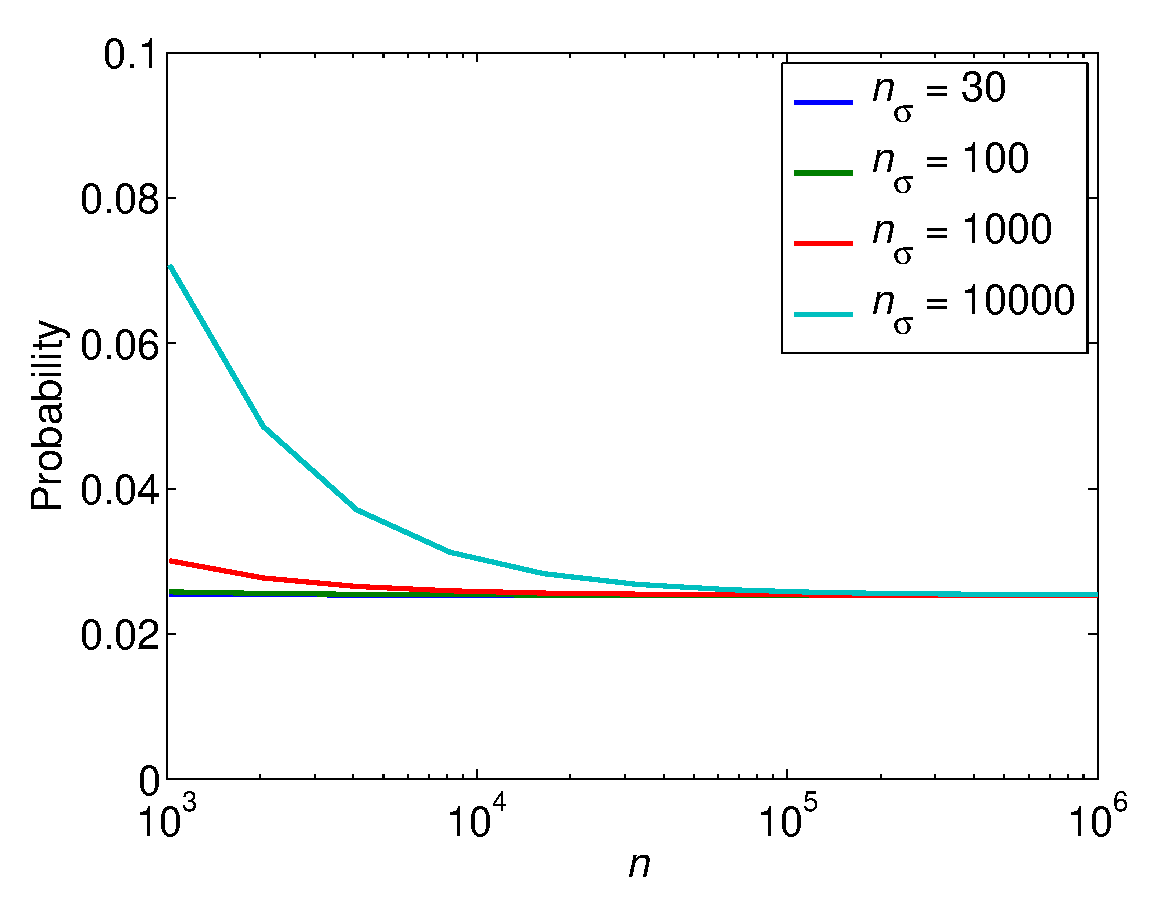
\includegraphics[width=3in]{probfailfig.eps}
\caption{The upper bound on the probability that $\hv_n \ge \hsigma^2$ in \eqref{probfail} for $\alpha_1 = 1 - \sqrt{95\%} \approx 2.5\%$ and $L=1.5$. \label{probfailfig}}
\end{figure}



%Consider a spacial case in (\ref{NB}), let $\Phi(-\frac{\sqrt{n}\epsilon}{\sigma})=\frac{A\varrho}{\sqrt{n}}=\frac{\alpha}{4}$, since $\varrho\leq (\kappa_{\max}+3)^{3/4}$,
%we can get the upper bound of $N_B(\epsilon,\alpha_1,\sigma_{\max},\varrho)$ by
%$$N_B(\epsilon,\alpha_1,\sigma_{\max},\varrho)\leq \max\{\frac{Z^2_{\alpha_1/4}\sigma^2_{\max}}{\epsilon^2},\frac{16A^2(\kappa_{\max}+3)^{3/2}}{\epsilon^2}\}$$

\section{Example}

Consider the case of the uniform probability distribution on $[0,1]$, i.e., $\rho=1$.  Define
\begin{equation} \label{exampleeq}
f(x) = \begin{cases} 1 + \sigma \sqrt{\frac{1-p}{p}}, & 0 \le x \le p,\\
1 - \sigma \sqrt{\frac{p}{1-p}}, & p < x \le 1,
\end{cases}
\end{equation}
where $p$ and $\sigma$ are parameters, with $0 < p < 1$.
Note that
\begin{align*}
\mu &= \int_0^1 g(x) \, \dif x = 1\\
\var(g) &= \int_0^1 [g(x)-\mu]^2 \, \dif x = \sigma^2 \frac{1-p}{p} p + \sigma^2 \frac{p}{1-p} (1-p) = \sigma^2, \\
\kappa = \kurt(g) &= \frac{1}{\sigma^4}\int_0^1 [g(x)-\mu]^4 \, \dif x = \left(\frac{1-p}{p}\right)^2 p + \left(\frac{p}{1-p} \right)^2 (1-p) \\
& = \frac{(1-p)^3 + p^3}{p(1-p)} = \frac{1-3p+3p^2}{p(1-p)} = \frac{1}{p(1-p)} - 3.
\end{align*}
Note that $\kappa$ ranges from a minimum of $1$, when $p=1/2$ to a maximum of $\infty$ when $p=0,1$.

\begin{figure}
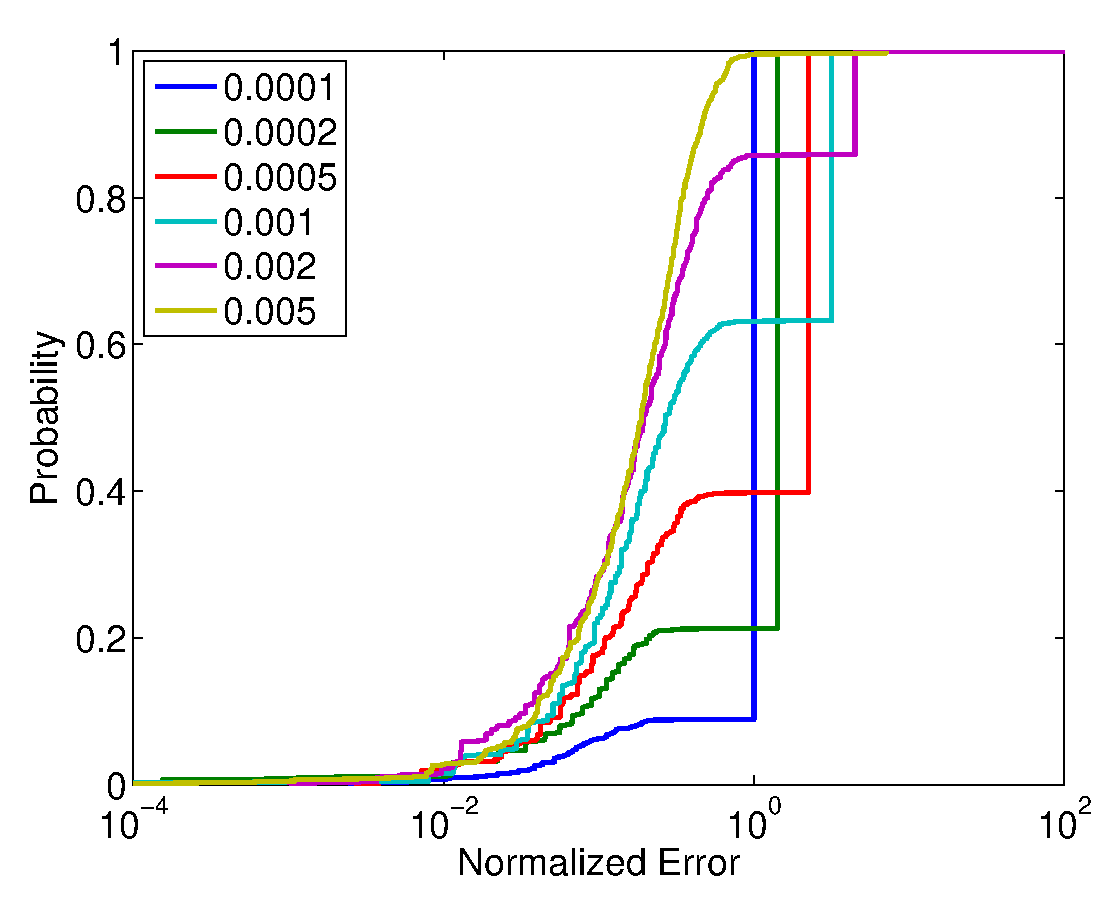
\includegraphics[width=3in]{NormalErrFig.eps}
\caption{Empirical distribution function of $\abs{\mu-\hmu_n}/\epsilon$ for example \eqref{exampleeq} with $\mu=\sigma=1$, $n_0=100$, $\kappa_{\max} = 3.2$, $\varepsilon=0.01$, and  $p=0.001, 0.002, 0.005, 0.01, 0.02, 0.05$ using the algorithm in Theorem \ref{mainadaptthm}. \label{normalerrfig}}
\end{figure}

Figure \ref{normalerrfig} shows the empirical distribution of the normalized error $\abs{\mu-\hmu_n}/\epsilon$, using $1000$ replications for a range of values of $p$.  As can be seen in this figure and in Table \ref{examptable}, the adaptive Monte Carlo method does poorly for very small values of $p$, which correspond to vary large values of the kurtosis.  However, even for values of the kurtosis above $\kappa_{\max}=3.2$ used in this example, the chance of meeting the error tolerance may be quite high.

\begin{table}
\caption{Kurtosis and probability of meeting the error tolerance for different values of $p$. \label{examptable}}
\[
\begin{array}{r|ccccccccccc}
p &   0.001 &    0.002 &    0.005 &     0.01 &     0.02 &     0.05 \\
\hline
\kappa &  998.00 &   498.00 &   198.01 &    98.01 &    48.02 &    18.05 \\
\hline
\Prob(\abs{\mu-\hmu_n} \le \varepsilon) &    8.70\% &    17.50\% &    39.20\% &    63.50\% &    86.40\% &    99.90\% \\
\end{array}
\]
\end{table}


\section{Questions}

Here are some questions that suggest themselves:

\begin{itemize}

\item Is this analysis above known already?  Is this the typical probabilistic setting?  Is it better to look at a randomized setting where one considers the expected value of the error?

\item Can this type of analysis be extended to randomized \emph{quasi-Monte Carlo} for finite dimension, $d$?  Infinite dimension?  In this latter case one needs some multilevel algorithm, but the specification of the levels perhaps could be deduced from the data.  One might also consider a case where the coordinate weights were not known a priori but needed to be estimated.

\item Is there already this kind of information-based complexity analysis where the number of operations is bounded above or below by the unknown scale of the problem (in this case the variance).  The IBC I know assumes that the scale is fixed, e.g., the function has variance one, norm one, etc.  Here we allow arbitrary scale, but do make assumptions on the nastiness (kurtosis).

\item Are there better inequalities than Chebyshev's inequality or the Berry-Esseen inequality that apply when $Z$ is the sum of i.i.d.\ random variables?  Some of the better known ones, like Hoeffding's inequality assume boundedness, which we cannot presume here.

\end{itemize}

\section*{Appendix of Useful Theorems}
\begin{theorem}[Chebyshev's Inequality] \label{Chebineqthm} Let $Z$ be any random variable with mean $\mu$ and variance $\sigma^2$.  Then for all $\alpha >0$, Chebyshev's inequality states that
\[
\Prob\left[\abs{Z-\mu} \ge \frac{\sigma}{\sqrt{\alpha}} \right] \le \alpha, \qquad \Prob\left[\abs{Z-\mu} < \frac{\sigma}{\sqrt{\alpha}} \right] \ge 1-\alpha.
\]
\end{theorem}
\begin{proof}To prove Chebyshev's inequality note that
\begin{equation*}
\sigma^2 = E[\abs{Z-\mu}^2] \ge \frac{\sigma^2}{\alpha} \Prob\left[\abs{Z-\mu} \ge \frac{\sigma}{\sqrt{\alpha}} \right],
\end{equation*}
and then divide both sides by $\sigma^2/\alpha$.
\end{proof}
The following theorem comes from \cite[Theorem 5.16, p. 168]{Pet95a}
\begin{theorem}[Non-uniform Berry-Esseen Inequality] \label{BE} Let $Y_1,\dots,Y_n$ be i.i.d.\ random variables.  Suppose that
\[
\mu=E(Y_i), \quad \var(Y_i)=\sigma^2>0, \quad \varrho=\frac{E\abs{Y_i - \mu}^3}{\sigma^3} < \infty.
\]
Then
\[
\abs{\Prob\left[\frac{1}{\sigma\sqrt{n}}\sum_{i=1}^{n}(Y_i-\mu)<x
\right]-\Phi(x)}\leq \frac{A \varrho}{\sqrt{n}}(1+\abs{x})^{-3}.
\] for all x,
where $\Phi$ is the cumulative distribution function of the standard normal random variable, and $A$ is some number satisfying $0.4097\leq A\leq 0.5600$.
\end{theorem}

\begin{theorem} \label{Varvarthm} Let $\hv_n$ be the sample variance as defined in \eqref{samplevar}.  It's variance is
\[
\var(\hv_n^2) = \frac{\sigma^4}{n} \left ( \kappa  - \frac{n-3}{n-1} \right),
\]
where $\kappa:= \kurt(g) = M_4(g)/\sigma^4(g)$ denotes the \emph{kurtosis}.
\end{theorem}
\begin{proof}The sample variance has mean $\sigma^2/n$.  To facilitate the derivation, let $Y_i=g(X_i) - \mu$.
\begin{align*}
\hv_n & =  \frac 1{n-1} \sum_{i=1}^n \left[Y_i- \left(\frac 1n \sum_{j=1}^n Y_j\right) \right]^2
=  \frac 1{n(n-1)}\left[ n \sum_{i=1}^n Y^2_i-  \sum_{j,k=1}^n Y_jY_k \right] \\
\hv_n^2 & = \frac 1{n^2(n-1)^2}\left[ n^2 \sum_{i,j=1}^n Y^2_i Y^2_j  - 2 n \sum_{i,j,k=1}^n Y^2_i Y_j Y_k +  \sum_{i,j,k,l=1}^n Y_iY_j Y_k Y_l\right] \\
E[ Y^2_i Y^2_j] & = \begin{cases} M_4, & i=j,\\
\sigma^4, & i \ne j,
\end{cases}\\
\sum_{i,j=1}^n E[Y^2_i Y^2_j]&= n M_4 + n(n-1)\sigma^4, \\
E[ Y^2_i Y_j Y_k] & = \begin{cases} M_4, & i=j=k,\\
\sigma^4, & i \ne j, j=k,\\
0, & j \ne k,
\end{cases} \\
\sum_{i,j,k=1}^n E[Y^2_i Y_j Y_k] &= nM_4  + n(n-1)\sigma^4 \\
E[ Y_i Y_j Y_k Y_l] & = \begin{cases} M_4, & i=j=k=l,\\
\sigma^4, & i, j, k, l \text{ have 2 distinct values},\\
0, & \text{otherwise},
\end{cases}\\
\sum_{i,j,k,l=1}^n E[Y_iY_j Y_k Y_l] &= n M_4 + 3n(n-1)\sigma^4 \\
E[\hv_n^2] & = \frac{ n^3[M_4 + (n-1)\sigma^4]  - 2 n^2 [M_4 + (n-1)\sigma^4] +  n[M_4 + 3(n-1)\sigma^4]} {n^2(n-1)^2} \\
& = \frac{ (n-1)M_4 + (n^2-2n+3)\sigma^4} {n(n-1)} \\
\var(\hv_n^2) & = E[\hv_n^2] - \left[E(\hv_n)\right]^2 = \frac{ (n-1)M_4 + (n^2-2n+3)\sigma^4} {n(n-1)} -\sigma^4\\
& = \frac{(n-1)M_4 + (-n+3)\sigma^4} {n(n-1)}= \frac{1}{n} \left ( M_4 - \frac{n-3}{n-1} \sigma^4 \right) = \frac{\sigma^4}{n} \left ( \kappa  - \frac{n-3}{n-1} \right).
\end{align*}
\end{proof}
\begin{theorem}[Single tailed Cantelli's inequality]\label{Can}
Let $Z$ be any random variable with mean $\mu$ and finite variance $\sigma^2$.  For any $a\geq 0$, it
follows that:
\[
\Prob[Z-\mu \geq a]\leq \frac{\sigma^2}{a^2+\sigma^2}.
\]
\end{theorem}
\begin{proof}Define the random variable
\[ S=\sign(Z - \mu - a) = \begin{cases} 1, & Z - \mu \geq a,\\ -1, & Z - \mu <a. \end{cases}
\]
From conditional probability it is known that
\begin{align*}
\sigma^2 &= \var(Z-\mu)=E[\var(Z-\mu|S)]+\var[E(Z-\mu|S)] \\
&\geq\var[E(Z-\mu|S)]= E[\{E(Z-\mu|S)\}^2]-[E\{E(Z-\mu|S)\}]^2 =  E[\{E(Z-\mu|S)\}^2]
\end{align*}
Since $E(Z-\mu)=0$, it follows that
\begin{equation*}
0= E[E(Z-\mu|S)]=E(X|S=1)\Prob(Z - \mu \geq a)+E(X|S=-1)\Prob(Z - \mu < a).
\end{equation*}
Also, it is clear that $E(Z - \mu|S=1) \ge a$, which implies that
\begin{equation*}
[E(Z - \mu|S=-1)]^2=\left[\frac{E(Z - \mu|S=1)\Prob(Z - \mu \geq a)}{\Prob(Z - \mu < a)}\right]^2\geq \left[\frac{a\Prob(Z - \mu \geq a)}{\Prob(Z - \mu < a)}\right]^2
\end{equation*}
Combining these results together yields
\begin{align*}
\sigma^2 & \ge E[\{E(Z-\mu|S)\}^2]\\
& =\{E(Z-\mu|S=1)\}^2 \Prob(Z - \mu \geq a) + \{E(Z-\mu|S=-1)\}^2 \Prob(Z - \mu < a) \\
& \ge a^2 \Prob(Z - \mu \geq a) + \left[\frac{a\Prob(Z - \mu \geq a)}{\Prob(Z - \mu < a)}\right]^2 \Prob(Z - \mu < a) \\
&= a^2 \left[\frac{ \Prob(Z - \mu \geq a)}{\Prob(Z - \mu < a)}\right] = a^2 \left[\frac{ \Prob(Z - \mu \geq a)}{1  - \Prob(Z - \mu \ge a)}\right]
\end{align*}
Solving this inequality for $\Prob(Z - \mu \geq a)$ completes the proof.
\end{proof}

\begin{prop}\label{propCant} Let $\hv_n$ be the sample variance of a function $g$ as defined in \eqref{samplevar}, and let $\kappa=\kurt(g)$.  Then
\begin{subequations} \label{sampvarbd}
\begin{gather}\label{sampvarup}
\Prob\left[\hv_n < \sigma^2 \left\{1 + \sqrt{\left ( \kappa  - \frac{n-3}{n-1}\right)\left(\frac{1-\alpha}{\alpha n}\right)}\right\} \right] \ge 1 - \alpha, \\
\label{sampvarlo}
\Prob\left[\hv_n > \sigma^2 \left\{1 - \sqrt{\left ( \kappa  - \frac{n-3}{n-1}\right)\left(\frac{1-\alpha}{\alpha n}\right)}\right\} \right] \ge 1 - \alpha.
\end{gather}
\end{subequations}
\end{prop}
\begin{proof}Choosing
$$a=\sigma^2\sqrt{\left(\kappa-\frac{n-3}{n-1}\right)\left(\frac{1-\alpha}{\alpha n}\right)} >0,
$$
we know from Cantelli's inequality (Theorem \ref{Can})  that
$$\Prob[\hv_n-\sigma^2 \geq
a]\leq\frac{\var(\hv_n)}{a^2+\var(\hv_n)}$$
\begin{align*}
\Prob\left[\hv_n-\sigma^2 \geq
\sigma^2\sqrt{\left(\kappa-\frac{n-3}{n-1}\right)\left(\frac{1-\alpha}{\alpha n}\right)} \right] & = \Prob\left[\hv_n-\sigma^2 \geq
a \right]\\
& \leq\frac{\var(\hv_n)}{a^2+\var(\hv_n)}\\
&= \frac{\frac{\sigma^4}{n}\left(\kappa - \frac{n-3}{n-1}\right)}{\frac{\sigma^4}{n}\left(\kappa - \frac{n-3}{n-1}\right)\left(\frac{1-\alpha}{\alpha}\right)+\frac{\sigma^4}{n}\left(\kappa - \frac{n-3}{n-1}\right)} \\
&=\frac{1}{\left(\frac{1-\alpha}{\alpha}\right)+1}=\alpha.
\end{align*}
Then \eqref{sampvarup} follows directly.  By a similar argument.
\begin{align*}
\Prob\left[\hv_n-\sigma^2 \le
- \sigma^2\sqrt{\left(\kappa-\frac{n-3}{n-1}\right)\left(\frac{1-\alpha}{\alpha n}\right)} \right] & = \Prob\left[\hv_n-\sigma^2 \le -a \right]\\
& = \Prob\left[(-\hv_n)-(-\sigma^2) \ge a \right]\\& \leq\frac{\var(-\hv_n)}{a^2+\var(-\hv_n)}= \frac{\var(\hv_n)}{a^2+\var(\hv_n)}\\
&= \frac{\frac{\sigma^4}{n}\left(\kappa - \frac{n-3}{n-1}\right)}{\frac{\sigma^4}{n}\left(\kappa - \frac{n-3}{n-1}\right)\left(\frac{1-\alpha}{\alpha}\right)+\frac{\sigma^4}{n}\left(\kappa - \frac{n-3}{n-1}\right)} \\
&=\frac{1}{\left(\frac{1-\alpha}{\alpha}\right)+1}=\alpha.
\end{align*}
Thus, \eqref{sampvarlo} follows as well.
\end{proof}

\bibliographystyle{spbasic}
\bibliography{FJH21,FJHown21}
\end{document}
